
On veut décorer le mur d’une salle de classe en y peignant un arbre stylisé, construit à partir 
de carrés de la façon suivante :
% \usepackage{array} is required
\begin{tabular}{|>{\centering\arraybackslash}p{0.25\linewidth}|>{\centering\arraybackslash}p{0.3\linewidth}|>{\centering\arraybackslash}p{0.35\linewidth}|}
\hline 
Étape 1 & Étape 2 & Étape 3 \\ 
\hline 
On part d’un carré de côté 80 cm, peint à partir du sol. & 
On construit deux autres carrés analogues, en laissant un vide en forme de triangle rectangle isocèle. &
Sur chaque carré construit à l’étape 1, on construit deux autres carrés 
à l’extérieur, comme à l’étape 1. \\ 
\hline 
 \definecolor{qqttzz}{rgb}{0.,0.2,0.6}
\begin{tikzpicture}[line cap=round,line join=round,>=triangle 45,x=1.0cm,y=1.0cm]
\clip(1.68,-3.24) rectangle (4.32,-0.72);
\fill[color=qqttzz,fill=qqttzz,fill opacity=1.0] (2.,-3.) -- (4.,-3.) -- (4.,-1.) -- (2.,-1.) -- cycle;
\draw [color=qqttzz] (2.,-3.)-- (4.,-3.);
\draw [color=qqttzz] (4.,-3.)-- (4.,-1.);
\draw [color=qqttzz] (4.,-1.)-- (2.,-1.);
\draw [color=qqttzz] (2.,-1.)-- (2.,-3.);
\end{tikzpicture}
& 
\definecolor{qqttzz}{rgb}{0.,0.2,0.6}
\begin{tikzpicture}[line cap=round,line join=round,>=triangle 45,x=1.0cm,y=1.0cm]
\clip(0.84,-3.22) rectangle (5.32,1.38);
\fill[color=qqttzz,fill=qqttzz,fill opacity=1.0] (2.,-3.) -- (4.,-3.) -- (4.,-1.) -- (2.,-1.) -- cycle;
\fill[color=qqttzz,fill=qqttzz,fill opacity=1.0] (2.,-1.) -- (3.,0.) -- (2.,1.) -- (1.,0.) -- cycle;
\fill[color=qqttzz,fill=qqttzz,fill opacity=1.0] (4.,-1.) -- (5.,0.) -- (4.,1.) -- (3.,0.) -- cycle;
\draw [color=qqttzz] (2.,-3.)-- (4.,-3.);
\draw [color=qqttzz] (4.,-3.)-- (4.,-1.);
\draw [color=qqttzz] (4.,-1.)-- (2.,-1.);
\draw [color=qqttzz] (2.,-1.)-- (2.,-3.);
\draw [color=qqttzz] (2.,-1.)-- (3.,0.);
\draw [color=qqttzz] (3.,0.)-- (2.,1.);
\draw [color=qqttzz] (2.,1.)-- (1.,0.);
\draw [color=qqttzz] (1.,0.)-- (2.,-1.);
\draw [color=qqttzz] (4.,-1.)-- (5.,0.);
\draw [color=qqttzz] (5.,0.)-- (4.,1.);
\draw [color=qqttzz] (4.,1.)-- (3.,0.);
\draw [color=qqttzz] (3.,0.)-- (4.,-1.);
\end{tikzpicture}
& \definecolor{qqttzz}{rgb}{0.,0.2,0.6}
\begin{tikzpicture}[line cap=round,line join=round,>=triangle 45,x=1.0cm,y=1.0cm]
\clip(-0.16,-3.26) rectangle (6.16,2.42);
\fill[color=qqttzz,fill=qqttzz,fill opacity=1.0] (2.,-3.) -- (4.,-3.) -- (4.,-1.) -- (2.,-1.) -- cycle;
\fill[color=qqttzz,fill=qqttzz,fill opacity=1.0] (1.,1.) -- (2.,1.) -- (2.,2.) -- (1.,2.) -- cycle;
\fill[color=qqttzz,fill=qqttzz,fill opacity=1.0] (0.,0.) -- (1.,0.) -- (1.,1.) -- (0.,1.) -- cycle;
\fill[color=qqttzz,fill=qqttzz,fill opacity=1.0] (4.,1.) -- (5.,1.) -- (5.,2.) -- (4.,2.) -- cycle;
\fill[color=qqttzz,fill=qqttzz,fill opacity=1.0] (5.,0.) -- (6.,0.) -- (6.,1.) -- (5.,1.) -- cycle;
\fill[color=qqttzz,fill=qqttzz,fill opacity=1.0] (2.,-1.) -- (3.,0.) -- (2.,1.) -- (1.,0.) -- cycle;
\fill[color=qqttzz,fill=qqttzz,fill opacity=1.0] (4.,-1.) -- (5.,0.) -- (4.,1.) -- (3.,0.) -- cycle;
\draw [color=qqttzz] (2.,-3.)-- (4.,-3.);
\draw [color=qqttzz] (4.,-3.)-- (4.,-1.);
\draw [color=qqttzz] (4.,-1.)-- (2.,-1.);
\draw [color=qqttzz] (2.,-1.)-- (2.,-3.);
\draw [color=qqttzz] (2.,1.)-- (2.,2.);
\draw [color=qqttzz] (2.,2.)-- (1.,2.);
\draw [color=qqttzz] (1.,2.)-- (1.,1.);
\draw [color=qqttzz] (1.,0.)-- (1.,1.);
\draw [color=qqttzz] (1.,1.)-- (0.,1.);
\draw [color=qqttzz] (0.,1.)-- (0.,0.);
\draw [color=qqttzz] (5.,1.)-- (5.,2.);
\draw [color=qqttzz] (5.,2.)-- (4.,2.);
\draw [color=qqttzz] (4.,2.)-- (4.,1.);
\draw [color=qqttzz] (6.,0.)-- (6.,1.);
\draw [color=qqttzz] (6.,1.)-- (5.,1.);
\draw [color=qqttzz] (5.,1.)-- (5.,0.);
\draw [color=qqttzz] (2.,-1.)-- (3.,0.);
\draw [color=qqttzz] (3.,0.)-- (2.,1.);
\draw [color=qqttzz] (2.,1.)-- (1.,0.);
\draw [color=qqttzz] (1.,0.)-- (2.,-1.);
\draw [color=qqttzz] (4.,-1.)-- (5.,0.);
\draw [color=qqttzz] (5.,0.)-- (4.,1.);
\draw [color=qqttzz] (4.,1.)-- (3.,0.);
\draw [color=qqttzz] (3.,0.)-- (4.,-1.);
\end{tikzpicture} \\ 
\hline 
\end{tabular} 

\begin{center}
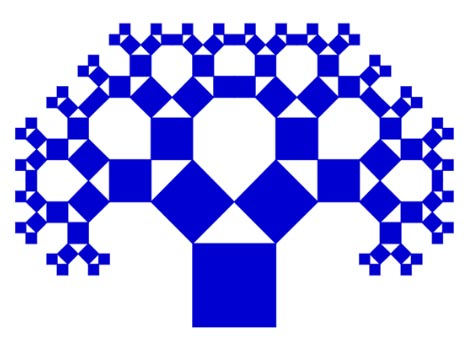
\includegraphics[scale=1]{Puis-19.jpg} 
\end{center}

On continue jusqu’à l’étape 4, en rajoutant chaque fois deux carrés sur ceux construits à l’étape d’avant. À partir de l’étape 5, on ne construit les nouveaux carrés que s’ils ne chevauchent pas les précédents. La figure ci-dessus représente l’arbre à l’étape 6.

\begin{enumerate}
\item Déterminer le côté des carrés construits à l’étape 2, à l’étape 3, à l’étape 7.
\item On réalise l’arbre, jusqu’à ce qu’il atteigne le plafond de la salle, haut de 3 mètres, et on le peint en bleu. Chaque pot de peinture contient 0,5 L, et chaque litre de peinture permet de recouvrir 3 mètres carrés. Marie affirme que quatre pots de peinture suffiront. A-t-elle raison ?
\end{enumerate}

